\documentclass[11pt,letterpaper]{article}

% Load some basic packages that are useful to have
% and that should be part of any LaTeX installation.
%
% be able to include figures
\usepackage{graphicx}
% get nice colors
\usepackage{xcolor}

% change default font to Palatino (looks nicer!)
\usepackage[latin1]{inputenc}
\usepackage{mathpazo}
\usepackage[T1]{fontenc}
% load some useful math symbols/fonts
\usepackage{latexsym,amsfonts,amsmath,amssymb}

% comfort package to easily set margins
\usepackage[top=1in, bottom=1in, left=1in, right=1in]{geometry}
\usepackage{hyperref}
\usepackage[all]{hypcap}
% control some spacings
%
% spacing after a paragraph
\setlength{\parskip}{.15cm}
% indentation at the top of a new paragraph
\setlength{\parindent}{0.0cm}


\begin{document}

\begin{center}
\Large
Ay190 -- Worksheet 02 Writeup\\
David Vartanyan\\
Date: \today
\end{center}

\section{Exercise 1}
We see single precision FP and possibly a poor recurrence relation contribute to excessive relative and absolute errors.

The absolute error at $n=15$ is $-3.65749328$. \newline The relative error at $n=15$ is $-5.24810071 \times 10^7$. See python file ws21.py on Github for the complete error table.

\section{Exercise 2}
I define a loop that takes a function of a function, the latter being the function we are trying to differentiate. Forward differencing is first order convergent since convergence goes as $(1/)^2$ on halving $h$. Central differencing is second order convergent since convergence goes as $(1/2)^2=1/4$ on halving $h$. \newline See Figure~\ref{fig:1} for a plot of both forward and central differencing convergences for $h$ and $h/2$.



\section{Exercise 3}

\begin{equation}
f(x_o-h)= f(x_o) - h \times f'(x_o) + h^2/2 \times f''(x_o) - h^3/6 \times f'''(x_o) + O(h^3)
\end{equation}
and
\begin{equation}
f(x_o+h)= f(x_o) + h \times f'(x_o) + h^2/2 \times f''(x_o) + h^3/6 \times f'''(x_o) + O(h^3)
\end{equation}
Adding and solving gives
\begin{equation}
f''(x_o) = \frac{f(x_o+h)+f(x_o-h) - 2 f(x_o)}{h^2} + O(h^2)
\end{equation}

\section{Exercise 4}
I discovered the $*=$ and $+=$ loops to perform the products and sums for the Lagrange interpolation. To get an output as a polynomial, I discovered the poly1d function searching stackoverflow.com.  Our Lagrange interpolation polynomial is\begin{multline}-1.072 \times 10^4 x^8 + 4.152 \times 10^4 x^7 - 6.613 \times 10^4 x^6 + 5.597 \times 10^4 x^5 - 2.715 \times 10^4 x^4 +\\
 7548 x^3 - 1113 x^2 + 66.38 x + 0.302 \end{multline}

For 4b, I simply read on scipy's library for piecewise linear and quadratic interpolation since the problem did not ask for code from scratch and encouraged learning scipy documentation.

See Figure~\ref{fig:2} for corresponding plots.
\section{Exercise 5}
The  difficult part of 5a was knowing how to express $x - x_i$, that is, for every $x$ we are interpolating over, finding the largest  element in our time [days] data $x_k$ 
that was less than $x$. Being very new to Python and after struggling without success, I took the professor's advice on the first day of class and turned to google. I want to make it abundantly clear that the corresponding 6 lines of code in my ws25a.py file (from lines 23-35 including comments) are from \href{http://matplotlib.1069221.n5.nabble.com/quot-Piecewise-Cubic-Hermite-Interpolating-Polynomial-quot-in-python-td24157.html}{``Piecewise Cubic Hermite Interpolating Polynomial in python''}.

Below I will summarize what I learned and how the code works:
First, some facts to know: this code uses multidimensional arrays of True, False and operates on those arrays. The logic is as follows:  $True - True = False = False - False$ while $False -True =True$.

The method is essentially to create an array of indices that has the same dimension as the array over which we are interpolating, which we call $k$. These indices correspond to the indices of $x_k$ defined above such that $x_k$ is the largest element less than the corresponding $x$ (that with the same index). 

This is achieved in quite a clever way. First, we convert our array of $x_i$ into $xx$, a $n \times mm$ array where $n$ is the dimension of the array of $x_i$ and $mm$ the dimension of our interpolation space $x$. This creates an array where each subsequent row is each subsequent time $x_i$, of which there are $n$ repeated $mm$ times. 
Then we impose the logic condition $xx>x$ to ask when are the elements of $x_i$ greater than those of $x$. This returns $z$, an $n \times mm$ array of True, False. 
Next we simply subtract adjacent columns. This returns an $n-1 \times mm$ array of True, False. We return True iff we transition from a column where $x_i < x$ to one where $x_i>x$, thus isolating the largest $x_i$ less than each correspond $x$! 
Last we simply use the python function argmax which runs through each column of $z$ and selects the first (and only) instance of True; for instance, the first 20 elements of $k$ are $0$ since the first 20 elements in our interpolating range (from $0 to .1$) all subtract $x_i-0$ from our data in this bin, following the Hermite formulation. The option $Axis=0$ parses through the columns (and $axis=1$ the rows). This returns $k$ defined above.

The problem with this code is that it breaks down at the right endpoint. First, it thought this was a relic of imposing $xx >x$ instead of using a $xx >= x$, since $1$ in our time data is not less than $1$ in the interpolation at our right endpoint. However, even if we correct for this, Hermite polynomial depends on the $k+1$ index which fails at the right endpoint. We correct for it by using a linear fit barely visible as a black line in our plot from $x=.99$ to $x=1$. The alternative would have been to extrapolate our slope $m$ to an extra value by assuming periodicity of the data and using Hermite interpolation for the right endpoint too.

5b was very straightforward and simply involved reading scipy documentation on the interpolate.splev() function. Natural simply indicates having the second derivative of our interpolation go to $0$ at the endpoints.

See Figure~\ref{fig:3} for corresponding plots.

\begin{figure}[bth]
\centering
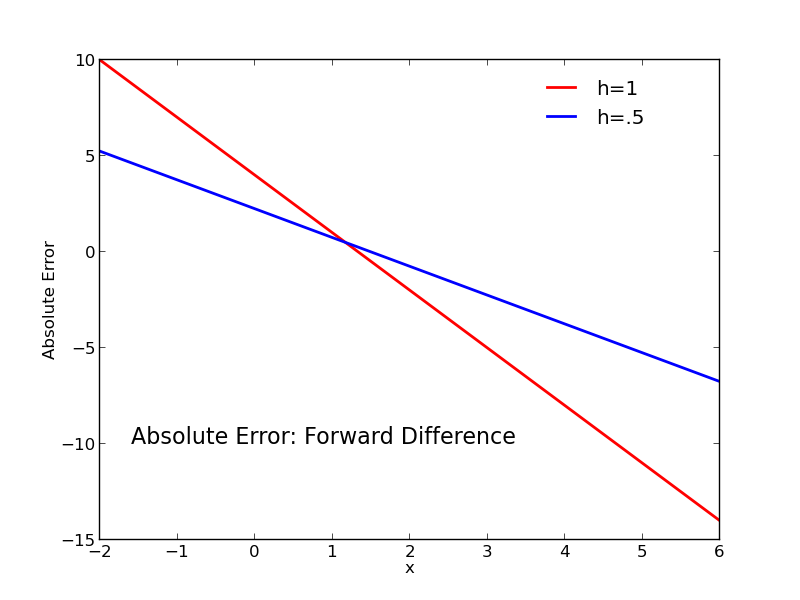
\includegraphics[width=.7\textwidth]{ws22f.png}
\caption{Forward Difference Convergence.}
\label{fig:1}
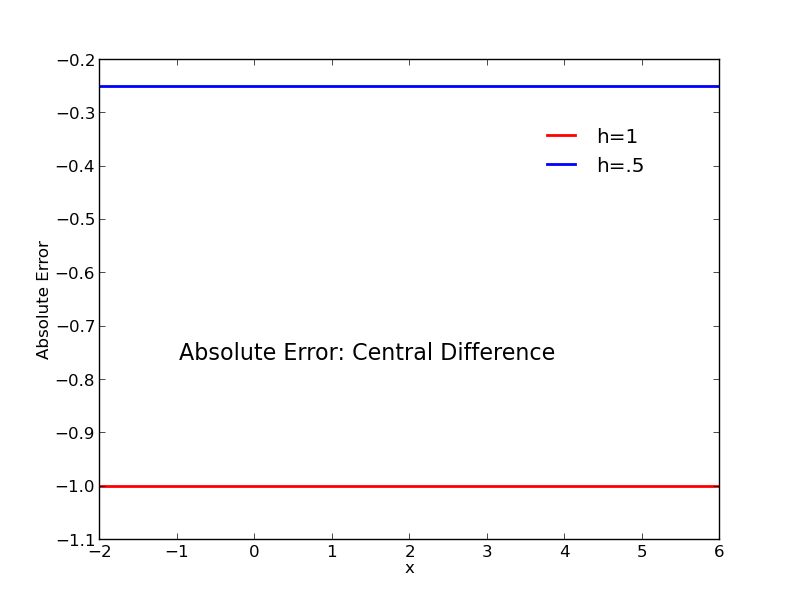
\includegraphics[width=0.7\textwidth]{ws22c.png}
\caption{Central Difference Convergence.}
\label{}
\end{figure}

\begin{figure}[bth]
\centering
\includegraphics[width=0.7\textwidth]{ws24a.png}
\caption{Lagrange Interpolation.}
\label{fig:2}
\includegraphics[width=0.7\textwidth]{ws24b.png}
\caption{Piecewise and Quadratic Interpolation}
\label{fig:2}
\end{figure}

\begin{figure}[bth]
\centering
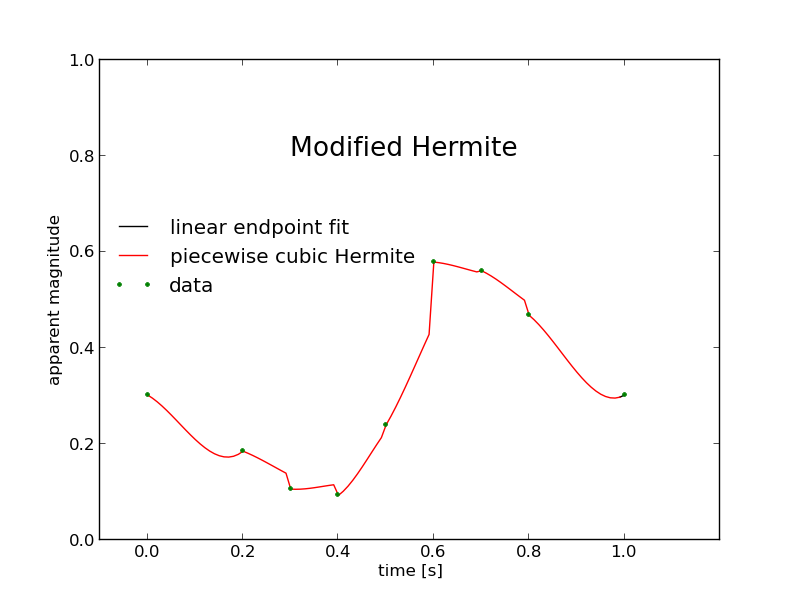
\includegraphics[width=0.7\textwidth]{ws25a.png}
\caption{Lagrange Interpolation.}
\label{fig:3}
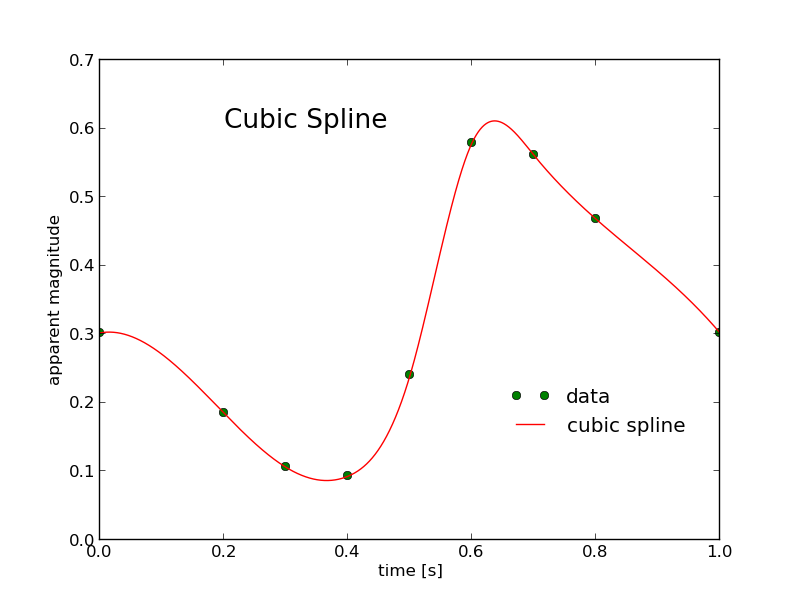
\includegraphics[width=0.7\textwidth]{ws25b.png}
\caption{Piecewise and Quadratic Interpolation}
\label{fig:3}
\end{figure}

\end{document}
